\addtocontents{xms}{\protect\addvspace{10pt}}
\chapter{Resolució de Xarxes Elèctriques} \label{sec:ch-xarxes-elec}
\index{metode@mètode dels nusos}
\section{Introducció}\label{sec:ch-xarxes-elec-intro}
S'explica en aquest capítol el
mètode dels nusos per a la resolució de xarxes elèctriques.

Quan tenim una xarxa elèctrica amb pocs components, sempre la podem resoldre fàcilment
utilitzant el mètode de les malles descrit en la secció \vref{sec:metode-malles}. No obstant això, quan la xarxa té molts components, quan està
 molt mallada o quan hi ha acoblaments magnètics entre diverses branques de la xarxa, és millor
 emprar un mètode sistemàtic per  resoldre-la, com ara el mètode dels nusos.

El mètode dels nusos serveix per resoldre xarxes, tant de corrent
continu com de corrent altern, on les càrregues estan definides pels
seus valors d'impedància o d'admitància; no és útil, per tant, per
resoldre problemes de flux de càrregues, on el que es coneix és la
potència absorbida per les càrregues.

Per tal d'utilitzar aquest mètode, les branques de la xarxa han d'estar
formades per algun dels següents components: \vspace{-1.5mm}
\begin{itemize}
   \item Font de tensió en sèrie amb una impedància.
   \item Font de corrent en paraŀlel amb una admitància.
   \item Impedància.
   \item Admitància.
   \item Acoblament magnètic entre branques.
   \item Transformador.\footnote{Cal substituir el transformador pel seu circuit equivalent format per impedàncies i    admitàncies. Vegeu la secció \ref{sec:trafo_reg}.}
\end{itemize}
\vspace{-1.5mm}

No és possible tenir branques d'impedància nuŀla --- curtcircuits --- o
branques amb fonts de tensió ideals  --- sense impedància sèrie.
Aquesta limitació es pot superar, tanmateix, substituint la
impedància nuŀla per dues impedàncies en sèrie  de valor
contrari, i introduint un nus fictici addicional en el punt d'unió
d'aquestes dues noves impedàncies. En la figura
\vref{pic:branca_nula}
 es representa gràficament aquesta substitució. \index{metode@mètode dels nusos!branques d'impedància
nuŀla}
\begin{center}
   \input{Imatges/Cap-ResXarxElec-Branques-Z0.pdf_tex}
    \captionof{figure}{Substitució de branques d'impedància nuŀla}
    \label{pic:branca_nula}
\end{center}

En el cas que tinguem branques amb una font de corrent ideal --- sense admitància en paraŀlel ---  també les haurem de substituir per una branca  formada per una font de corrent amb una admitància en paraŀlel, i una branca fictícia en paraŀlel amb una admitància de valor contrari. En la figura \vref{pic:branca_J_nula} es representa gràficament aquesta substitució.
\begin{center}
	\input{Imatges/Cap-ResXarxElec-Branques-Y0.pdf_tex}
	\captionof{figure}{Substitució de branques amb una font de corrent ideal}
	\label{pic:branca_J_nula}
\end{center}

Per ajudar-nos en l'explicació d'aquest mètode de resolució de xarxes, farem
ús de l'exemple de la figura \vref{pic:metode_nusos}. Els valors dels components d'aquest
circuit són:
\begin{align*}
   \cmplx{E}_1 &= \qtypd{200}{0}{V} & R_1 &= \qty{10}{\ohm} &
   \cmplx{E}_2 &= \qtypd{50}{0}{V}  & \cmplx{X}_2 &= \complexqty{j20}{\ohm} &
   \cmplx{X}_3 &= \complexqty{j5}{\ohm} \\
   R_4 &= \qty{20}{\ohm} & \cmplx{J}_5 &= \qtypd{4}{0}{A} &
   R_5 &= \qty{10}{\ohm} & \cmplx{X}\ped{M} &= \complexqty{j5}{\ohm}
\end{align*}

\begin{center}
\vspace{-4mm}
    \input{Imatges/Cap-ResXarxElec-Circuit-Graf.pdf_tex}
   \captionof{figure}{Resolució de xarxes elèctriques pel mètode dels nusos} \label{pic:metode_nusos}
\end{center}

\index{graf orientat}En primer lloc, a partir de la xarxa elèctrica
cal representar-ne el graf orientat (figura \vref{pic:metode_nusos} dreta) seguint els passos següents:
\begin{dingautolist}{'312}
   \item Es representen les connexions de les branques mitjançant línies, sense dibuixar-hi cap component elèctric.
   \item Es dona un sentit a aquestes branques, dibuixant-hi fletxes. Aquestes fletxes representen els sentits assignats als corrents i a les diferències de potencial entre nusos.
   \item Es numeren tots els nusos de forma consecutiva, començant pel número 0; el nus 0 s'anomena nus de potencial zero o de referència.
\index{nus!de potencial zero}\index{nus!de referència}
   \item Es numeren totes les branques de forma consecutiva, començant pel número 1.
\end{dingautolist}

\index{metode@mètode dels nusos!nombre de nusos}\index{metode@mètode
dels nusos!nombre de branques}Es defineixen a continuació els dos
paràmetres bàsics d'aquest mètode, $n$ i $b$; aquests dos valors
defineixen les dimensions dels vectors i matrius que es veuran més
endavant:
\begin{list}{}
   {\setlength{\labelwidth}{7mm} \setlength{\leftmargin}{9mm} \setlength{\labelsep}{2mm}}
   \item[$n$] Nombre de nusos de la xarxa, sense comptar el nus de referència.

   En el nostre exemple tenim:
   \[ n=2 \]

   \item[$b$] Nombre de branques de la xarxa.

   En el nostre exemple tenim:
   \[ b=5 \]
\end{list}

\section{Mètode general de resolució}

\index{metode@mètode dels nusos!cas general}Quan hi ha acoblaments
magnètics entre branques de la xarxa hem d'utilitzar el mètode
general de resolució, descrit a continuació.

En primer lloc, a partir dels valors dels components de la xarxa, formem les matrius i vectors següents (se'n donen les  dimensions entre claus):
\begin{list}{}
{\setlength{\labelwidth}{20mm} \setlength{\leftmargin}{22mm} \setlength{\labelsep}{2mm}}
   \item[$\boldsymbol{A}\{n\times b\}$] \index{matriu!d'incidència de nusos $\boldsymbol{A}$}Matriu d'incidència de nusos. Cada columna representa una branca en ordre creixent d'esquerra a dreta, i cada fila representa un nus --- sense comptar el de referència --- en ordre creixent de dalt a baix. Cada branca del graf orientat omple la columna corresponent de la matriu $\boldsymbol{A}$ amb els valors 0, 1 o $-1$ segons el criteri següent:
   \begin{list}{}
   {\setlength{\labelwidth}{7mm} \setlength{\leftmargin}{9mm} \setlength{\labelsep}{2mm}}
      \item[1:]  si la branca surt del nus.
      \item[$-1$:] si la branca va a parar al nus.
      \item[0:]  si la branca ni surt ni va a parar al nus.
   \end{list}
   Els termes «surt» i «va a parar» s'han d'entendre segons les fletxes dibuixades en les branques del graf orientat. Les connexions al nus de referència no apareixen en la matriu $\boldsymbol{A}$.

   En el nostre exemple tenim:
   \[
      \boldsymbol{A} = \left(\begin{array}{rrrrr} -1 & 1  & 0 &  1 & 0 \\  0 & -1 & 1 & -1 & -1
                   \end{array} \right)
   \]

   \item[$\mcmplx{Z}\ped{B}\{b\times b\}$] \index{matriu!d'impedàncies de branca $\mcmplx{Z}\ped{B}$}Matriu d'impedàncies de branca. Els elements de la diagonal estan formats per les impedàncies de les respectives branques, i els elements de fora de la diagonal estan formats per les impedàncies dels acoblaments magnètics entre cada parell de branques.

   Els acoblaments magnètics poden ser positius o negatius, depenent
    de la posició dels punts homòlegs de les inductàncies i del sentit
    de les branques del graf orientat. L'acoblament és positiu quan les
    fletxes de les dues branques acoblades es dirigeixen cap als seus punts
    homòlegs respectius, o quan les dues fletxes se n'allunyen; en canvi,
    l'acoblament és negatiu quan una de les fletxes de les dues branques
    acoblades es dirigeix cap al seu punt homòleg i l'altra se n'allunya.
    \index{acoblament magnètic}

   En el nostre exemple tenim:
   \[
      \mcmplx{Z}\ped{B} = \begin{pmatrix}
            10 & 0 & 0 & 0 & 0 \\
            0 & \ju 20 & \ju 5 & 0 & 0 \\
            0 & \ju 5 & \ju 5 & 0 & 0 \\
            0 & 0 & 0 & 20 & 0 \\
            0 & 0 & 0 & 0 & 10
      \end{pmatrix}\unit{\,\ohm}
   \]

   \item[$\mcmplx{E}'\ped{B}\{b\}$] \index{vector!de forces electromotrius $\mcmplx{E}'\ped{B}$}Vector columna de forces electromotrius de branca. Els elements d'aquest vector estan formats per les forces electromotrius de les fonts de tensió de les respectives branques.

El signe de cada força electromotriu és positiu si el seu sentit coincideix amb el sentit de la fletxa de la branca corresponent del graf orientat, i negatiu en cas contrari.

   En el nostre exemple tenim:
   \[
      \mcmplx{E}'\ped{B} = \begin{pmatrix} 200 \\ -50 \\ 0 \\ 0 \\ 0 \end{pmatrix}\unit{\,V}
   \]

   \item[$\mcmplx{J}'\ped{B}\{b\}$] \index{vector!d'intensivitats de branca $\mcmplx{J}'\ped{B}$}Vector columna d'intensivitats de branca. Els elements d'aquest vector estan formats per les intensivitats de les fonts de corrent de les respectives branques.

El signe de cada intensivitat és positiu si el seu sentit coincideix amb el sentit de la fletxa de la branca corresponent del graf orientat, i negatiu en cas contrari.

   En el nostre exemple tenim:
   \[
      \mcmplx{J}'\ped{B} = \begin{pmatrix} 0 \\ 0 \\ 0 \\ 0 \\ 4 \end{pmatrix}\unit{\,A}
   \]

\end{list}

A partir de les dades anteriors formem ara les diverses matrius i
vectors que ens permetran resoldre la xarxa, això és, trobar les
tensions de les branques i els corrents que hi circulen. Aquestes
matrius i vectors són (se'n donen les dimensions entre claus):

\begin{list}{}
{\setlength{\labelwidth}{20mm} \setlength{\leftmargin}{22mm} \setlength{\labelsep}{2mm}}
   \item[$\mcmplx{Y}\ped{B}\{b\times b\}$] \index{matriu!d'admitàncies de branca $\mcmplx{Y}\ped{B}$}Matriu d'admitàncies de branca. És definida per la relació següent:
   \begin{equation}
      \mcmplx{Y}\ped{B} = \mcmplx{Z}\ped{B}^{-1}
   \end{equation}

   En el nostre exemple tenim:
   \[
      \mcmplx{Y}\ped{B} = \begin{pmatrix}
            10 & 0 & 0 & 0 & 0 \\
            0 & \ju 20 & \ju 5 & 0 & 0 \\
            0 & \ju 5 & \ju 5 & 0 & 0 \\
            0 & 0 & 0 & 20 & 0 \\
            0 & 0 & 0 & 0 & 10
      \end{pmatrix} ^{-1}\unit{S} =
      \begin{pmatrix}
            \frac{1}{10} & 0 & 0 & 0 & 0 \\
            0 & -\ju\frac{1}{15} & \ju\frac{1}{15} & 0 & 0 \\[2mm]
            0 & \ju\frac{1}{15} & -\ju\frac{4}{15} & 0 & 0 \\[2mm]
            0 & 0 & 0 & \frac{1}{20} & 0 \\[2mm]
            0 & 0 & 0 & 0 & \frac{1}{10}
      \end{pmatrix}\,\unit{S}
   \]

   \item[$\mcmplx{J}\ped{B}\{b\}$] \index{vector!d'intensivitats equivalents de branca $\mcmplx{J}\ped{B}$}Vector columna d'intensivitats  equivalents de branca. És definit per la relació següent:
   \begin{equation}
      \mcmplx{J}\ped{B} = \mcmplx{J}'\ped{B}  + \mcmplx{Y}\ped{B} \,\mcmplx{E}'\ped{B}
   \end{equation}

   En el nostre exemple tenim:
   \[
      \mcmplx{J}\ped{B} =
      \begin{pmatrix} 0 \\ 0 \\ 0 \\ 0 \\ 4 \end{pmatrix}\,\unit{A} +
       \begin{pmatrix}
            \frac{1}{10} & 0 & 0 & 0 & 0 \\
            0 & -\ju\frac{1}{15} & \ju\frac{1}{15} & 0 & 0 \\[2mm]
            0 & \ju\frac{1}{15} & -\ju\frac{4}{15} & 0 & 0 \\[2mm]
            0 & 0 & 0 & \frac{1}{20} & 0 \\[2mm]
            0 & 0 & 0 & 0 & \frac{1}{10}
      \end{pmatrix}\,\unit{S} \cdot
      \begin{pmatrix} 200 \\ -50 \\ 0 \\ 0 \\ 0 \end{pmatrix}\,\unit{V} =
      \begin{pmatrix}
            20 \\[2mm]
             \ju \frac{10}{3} \\[2mm]
             -\ju \frac{10}{3} \\[2mm]
             0 \\[2mm]
              4
      \end{pmatrix}\,\unit{A}
   \]

   \item[$\mcmplx{Y}\ped{N}\{n\times n\}$] \index{matriu!d'admitàncies de nus $\mcmplx{Y}\ped{N}$}Matriu d'admitàncies de nus. És definida per la relació següent:
   \begin{equation}
      \mcmplx{Y}\ped{N} = \boldsymbol{A} \mcmplx{Y}\ped{B}
      \transp{\boldsymbol{A}}
   \end{equation}

   En el nostre exemple tenim:
   {\fontsize{10pt}{10pt}\selectfont
   \[
      \mcmplx{Y}\ped{N} =
      \left(\begin{array}{rrrrr} -1 & 1  & 0 &  1 & 0 \\  0 & -1 & 1 & -1 & -1
      \end{array}\right) \cdot
      \begin{pmatrix}
            \frac{1}{10} & 0 & 0 & 0 & 0 \\
            0 & -\ju\frac{1}{15} & \ju\frac{1}{15} & 0 & 0 \\[2mm]
            0 & \ju\frac{1}{15} & -\ju\frac{4}{15} & 0 & 0 \\[2mm]
            0 & 0 & 0 & \frac{1}{20} & 0 \\[2mm]
            0 & 0 & 0 & 0 & \frac{1}{10}
      \end{pmatrix}\,\unit{S} \cdot
      \left(\begin{array}{rr} -1 & 0 \\ 1  & -1 \\  0 & 1 \\ 1 & -1 \\ 0 & -1
      \end{array}\right)
       =
      \begin{pmatrix}
            \frac{\complexnum{9 - j 4}}{60} & \frac{\complexnum{-3 + j 8}}{60} \\[2mm]
            \frac{\complexnum{-3 + j 8}}{60} & \frac{\complexnum{9 - j 28}}{60}
      \end{pmatrix}\,\unit{S}
      \label{eq:yn}
   \]}

   \item[$\mcmplx{J}\ped{N}\{n\}$] \index{vector!d'intensivitats de nus $\mcmplx{J}\ped{N}$}Vector columna d'intensivitats de nus. És definit per la relació següent:
   \begin{equation}
      \mcmplx{J}\ped{N} = - \boldsymbol{A} \,\mcmplx{J}\ped{B}
   \end{equation}

   En el nostre exemple tenim:
   \[
      \mcmplx{J}\ped{N} = -
      \left(\begin{array}{rrrrr} -1 & 1  & 0 &  1 & 0 \\  0 & -1 & 1 & -1 & -1
      \end{array}\right) \cdot
      \begin{pmatrix}
            20 \\[2mm]
             \ju \frac{10}{3} \\[2mm]
             -\ju \frac{10}{3} \\[2mm]
             0 \\[2mm]
              4
      \end{pmatrix}\,\unit{A}
      =
      \begin{pmatrix}
            20 - \ju \frac{10}{3} \\[2mm]
            4 + \ju \frac{20}{3}
      \end{pmatrix}\unit{\,A}
   \]

   \item[$\mcmplx{V}\ped{N}\{n\}$] \index{vector!de potencials de nus $\mcmplx{V}\ped{N}$}Vector columna de potencials de nus. És definit per la relació següent:
   \begin{equation}
      \mcmplx{Y}\ped{N} \mcmplx{V}\ped{N} = \mcmplx{J}\ped{N} \quad\Rightarrow\quad
      \mcmplx{V}\ped{N} = \mcmplx{Y}\ped{N}^{-1} \mcmplx{J}\ped{N} \label{eq:vn}
   \end{equation}

   Els elements d'aquest vector són els potencials de cada nus de la xarxa respecte del nus de referència.

   En el nostre exemple tenim:
   \[
      \mcmplx{V}\ped{N} =
      \begin{pmatrix}
            \frac{\complexnum{ 9 - j 4}}{60} & \frac{\complexnum{-3 + j 8}}{60} \\[2mm]
            \frac{\complexnum{-3 + j 8}}{60} & \frac{\complexnum{9 - j 28}}{60}
      \end{pmatrix} ^{-1}\unit{\ohm} \cdot
      \begin{pmatrix}
            20 - \ju \frac{10}{3} \\[2mm]
            4 + \ju \frac{20}{3}
      \end{pmatrix}\,\unit{A}
      =
      \begin{pmatrix}
            \frac{\complexnum{15430 + j 2295}}{101} \\[2mm]
            \frac{\complexnum{3390 + j 2085}}{101}
      \end{pmatrix}\,\unit{V}
      \label{eq:vn_exemp}
   \]

   \item[$\mcmplx{U}\ped{B}\{b\}$] \index{vector!de tensions de branca $\mcmplx{U}\ped{B}$}Vector columna de tensions de branca. És definit per la relació següent:
   \begin{equation}
      \mcmplx{U}\ped{B} = \transp{\boldsymbol{A}} \mcmplx{V}\ped{N} \label{eq:ur}
   \end{equation}

   Aquesta és la solució buscada pel que fa a les tensions de les branques de la xarxa.

   En el nostre exemple tenim:
   \[
      \mcmplx{U}\ped{B} =
      \left(\begin{array}{rr} -1 & 0 \\ 1  & -1 \\  0 & 1 \\ 1 & -1 \\ 0 & -1
      \end{array}\right) \cdot
      \begin{pmatrix}
            \frac{\complexnum{15430 + j 2295}}{101} \\[2mm]
            \frac{\complexnum{3390 + j 2085}}{101}
      \end{pmatrix}\,\unit{V} =
      \begin{pmatrix}
           \frac{\complexnum{ -15430 - j 2295}}{101} \\[2mm]
           \frac{\complexnum{12040 + j 210}}{101}  \\[2mm]
           \frac{\complexnum{3390 + j 2085}}{101} \\[2mm]
           \frac{\complexnum{ 12040 + j 210}}{101}  \\[2mm]
           \frac{\complexnum{ -3390 - j 2085}}{101}
      \end{pmatrix}\,\unit{V}
   \]

   \item[$\mcmplx{I}\ped{B}\{b\}$] \index{vector!de corrents de branca $\mcmplx{I}\ped{B}$} Vector columna de corrents de branca. És definit per la relació següent:
   \begin{equation}
      \mcmplx{I}\ped{B} = \mcmplx{Y}\ped{B} \,\mcmplx{U}\ped{B} + \mcmplx{J}\ped{B} \label{eq:ir}
   \end{equation}

   Aquesta és la solució buscada pel que fa als corrents de les branques de la xarxa.

   En el nostre exemple tenim:
   \[
   \mcmplx{I}\ped{B} =
   \begin{pmatrix}
         \frac{1}{10} & 0 & 0 & 0 & 0 \\[2mm]
         0 & -\ju \frac{1}{15} & \ju \frac{1}{15} & 0 & 0 \\[2mm]
         0 & \ju \frac{1}{15} & -\ju \frac{4}{15} & 0 & 0 \\[2mm]
         0 & 0 & 0 & \frac{1}{20} & 0 \\[2mm]
         0 & 0 & 0 & 0 & \frac{1}{10}
   \end{pmatrix}\,\unit{S} \cdot
   \begin{pmatrix}
           \frac{\complexnum{ -15430 - j 2295}}{101} \\[2mm]
           \frac{\complexnum{12040 + j 210}}{101}  \\[2mm]
           \frac{\complexnum{3390 + j 2085}}{101} \\[2mm]
           \frac{\complexnum{ 12040 + j 210}}{101}  \\[2mm]
           \frac{\complexnum{ -3390 - j 2085}}{101}
      \end{pmatrix}\,\unit{V}
   + \begin{pmatrix}
         20 \\[2mm]
         \ju \frac{10}{3} \\[2mm]
         -\ju \frac{10}{3} \\[2mm]
         0 \\[2mm]
         4
      \end{pmatrix}\,\unit{A} =
     \begin{pmatrix}
      \frac{\complexnum{ 954 - j 459}}{202} \\[2mm]
      \frac{\complexnum{-250 - j 480}}{202}  \\[2mm]
      \frac{\complexnum{1084 - j 876}}{202} \\[2mm]
      \frac{\complexnum{1204 + j 21}}{202}  \\[2mm]
      \frac{\complexnum{130 - j 417}}{202}
   \end{pmatrix}\,\unit{A}
   \]

\end{list}

Es fa un resum, per acabar, dels passos a seguir per tal de resoldre una
xarxa elèctrica mitjançant el mètode dels nusos:
\begin{dingautolist}{'312}
   \item Es representa el graf orientat associat a la xarxa, i es numeren tots els seus nusos i totes les seves branques.
   \item A partir del graf orientat i dels elements de la xarxa, es formen les matrius $\boldsymbol{A}$ i $\mcmplx{Z}\ped{B}$, i els vectors $\mcmplx{E}\ped{B}'$ i $\mcmplx{J}\ped{B}'$.
   \item Es calculen les matrius $\mcmplx{Y}\ped{B}$ i $\mcmplx{Y}\ped{N}$, i els vectors $\mcmplx{J}\ped{B}$ i $\mcmplx{J}\ped{N}$.
   \item Finalment es calculen els vectors $\mcmplx{V}\ped{N}$, $\mcmplx{U}\ped{B}$ i $\mcmplx{I}\ped{B}$.
\end{dingautolist}


\begin{exemple}[\XarxaAmbAcobl{} \hyperlink{exemple:XarxaAmbAcobl}{\large\textcolor{NavyBlue}{(\faPython)}}]\label{ex:XarxaAmbAcobl}
	\addcontentsxms{\XarxaAmbAcobl}
    Es tracta de resoldre la xarxa següent pel mètode dels nusos; cal
    tenir en compte que a més de la càrrega Q8, els generadors G1, G2 i
    G3 també estan units a terra (nus 0 de referència), i que hi ha un
    acoblament magnètic M entre les línies L5 i L6. Es calcularà també
    la potència cedida pels tres generadors G1, G2 i G3, la potència
    absorbida per la càrrega Q8 i la potència perduda en la resta de
    components de la xarxa.
    \begin{center}
       \input{Imatges/Cap-ResXarxElec-Exemple-Circuit.pdf_tex}
    \end{center}

    Els valors dels components d'aquesta xarxa, expressats en per unitat són:
    \begin{align*}
       G1 &:\; \cmplx{e}_1 = \num{1,1} \qquad\qquad\;\;\, \cmplx{z}_1 = \complexnum{j 0,25} & L4 &:\; \cmplx{z}_4 = \complexnum{j 0,10} & T7 &:\; \cmplx{z}_7 = \complexnum{j 0,16} \quad\quad m_7=1:1\\*[3mm]
       G2 &:\; \cmplx{e}_2 = \complexnum{1,05+j0,10} \quad \cmplx{z}_2 = \complexnum{j 0,20} & L5 &:\; \cmplx{z}_5 = \complexnum{j 0,405}  & Q8 &:\; \cmplx{j}_8 = \complexnum{2-j0,9} \quad \cmplx{z}_8 = \complexnum{-j25} \\[3mm]
       G3 &:\; \cmplx{e}_3 = \complexnum{1,08+j0,12} \quad \cmplx{z}_3 = \complexnum{j 0,25} & L6 &:\; \cmplx{z}_6 = \complexnum{j 0,50} & M &:\; \cmplx{x}_M = \complexnum{j0,05}\; \text{(entre L5 i L6)}
    \end{align*}

    Començarem dibuixant el graf orientat associat a la xarxa, i formant la matriu $\boldsymbol{A}$.
    \begin{center}
         \input{Imatges/Cap-ResXarxElec-Exemple-Graf.pdf_tex}
    \end{center}

    \[
       \boldsymbol{A} = \left( \begin{array}{rrrrrrrr}
         -1 & 0 & 0 & 0 & 0 & 0 & 1 & 0 \\
         0 & -1 & 0 & 0 & 1 & 1 & -1 & 0 \\
         0 & 0 & -1 & 1 & 0 & -1 & 0 & 0 \\
         0 & 0 & 0 & -1 & -1 & 0 & 0 & 1
       \end{array}\right)
    \]

    Formem a continuació la matriu $\mcmplx{Z}\ped{B}$ i els vectors $\mcmplx{J}\ped{B}'$ i $\mcmplx{E}\ped{B}'$ (tots els valors en per unitat):

    \[
       \mcmplx{Z}\ped{B} =
       \begin{pmatrix}
         \complexnum{j 0,25} & 0 & 0 & 0 & 0 & 0 & 0 & 0 \\
         0 & \complexnum{j 0,20} & 0 & 0 & 0 & 0 & 0 & 0 \\
         0 & 0 & \complexnum{j 0,25} & 0 & 0 & 0 & 0 & 0 \\
         0 & 0 & 0 & \complexnum{j 0,10} & 0 & 0 & 0 & 0 \\
         0 & 0 & 0 & 0 & \complexnum{j 0,405} & \complexnum{j 0,05} & 0 & 0 \\
         0 & 0 & 0 & 0 & \complexnum{j 0,05} & \complexnum{j 0,50} & 0 & 0 \\
         0 & 0 & 0 & 0 & 0 & 0 & \complexnum{j 0,16} & 0 \\
         0 & 0 & 0 & 0 & 0 & 0 & 0 & \complexnum{-j 25}
       \end{pmatrix}
    \]

    \[
       \mcmplx{J}\ped{B}' =
       \begin{pmatrix}
        0 \\
        0 \\
        0 \\
        0 \\
        0 \\
        0 \\
        0 \\
        \complexnum{2 - j 0,9}
       \end{pmatrix}
       \qquad \qquad
       \mcmplx{E}\ped{B}' =
       \begin{pmatrix}
        \num{1,1} \\
        \complexnum{1,05 + j 0,10} \\
        \complexnum{1,08 + j 0,12} \\
        0 \\
        0 \\
        0 \\
        0 \\
        0
       \end{pmatrix}
    \]

    Calculem ara la matriu $\mcmplx{Y}\ped{B}=\mcmplx{Z}\ped{B}^{-1}$ i el vector $\mcmplx{J}\ped{B} = \mcmplx{J}\ped{B}' + \mcmplx{Y}\ped{B} \,\mcmplx{E}\ped{B}'$  (tots els valors en per unitat):

    \[
       \mcmplx{Y}\ped{B} =
       \begin{pmatrix}
         -\ju 4 & 0 & 0 & 0 & 0 & 0 & 0 & 0 \\
         0 & -\ju 5 & 0 & 0 & 0 & 0 & 0 & 0 \\
         0 & 0 & -\ju 4 & 0 & 0 & 0 & 0 & 0 \\
         0 & 0 & 0 & -\ju 10 & 0 & 0 & 0 & 0 \\
         0 & 0 & 0 & 0 & \complexnum{-j 2,5} & \complexnum{j 0,25} & 0 & 0 \\
         0 & 0 & 0 & 0 & \complexnum{j 0,25} & \complexnum{-j 2,025} & 0 & 0 \\
         0 & 0 & 0 & 0 & 0 & 0 & \complexnum{-j 6,25} & 0 \\
         0 & 0 & 0 & 0 & 0 & 0 & 0 & \complexnum{j 0,04}
       \end{pmatrix}
       \qquad
       \mcmplx{J}\ped{B} =
       \begin{pmatrix}
        \complexnum{-j 4,4} \\
        \complexnum{0,5 - j 5,25} \\
        \complexnum{0,48 - j 4,32} \\
        0 \\
        0 \\
        0 \\
        0 \\
        \complexnum{2 - j 0,9}
       \end{pmatrix}
    \]

    Continuem amb el càlcul de la matriu $\mcmplx{Y}\ped{N} =
    \boldsymbol{A} \mcmplx{Y}\ped{B} \transp{\boldsymbol{A}}$ i dels
    vectors $\mcmplx{J}\ped{N} = - \boldsymbol{A} \mcmplx{J}\ped{B}$ i
    $\mcmplx{V}\ped{N} = \mcmplx{Y}\ped{N}^{-1} \mcmplx{J}\ped{N}$ (tots
    els valors en per unitat):
    \[
       \mcmplx{Y}\ped{N} =
       \begin{pmatrix}
         \complexnum{-j 10,25} & \complexnum{j 6,25} & 0 & 0 \\
         \complexnum{j 6,25} & \complexnum{-j 15,275} & \complexnum{j 1,775} & \complexnum{j 2,25} \\
         0 & \complexnum{j 1,775 }& \complexnum{-j 16,025} & \complexnum{j 10,25} \\
         0 & \complexnum{j 2,25} & \complexnum{j 10,25} & \complexnum{-j 12,46}
       \end{pmatrix}
    \]
    \qquad
    \[
       \mcmplx{J}\ped{N} =
       \begin{pmatrix}
        \complexnum{-j 4,4} \\
        \complexnum{0,5 - j 5,25} \\
       \complexnum{ 0,48 - j 4,32} \\
        \complexnum{-2 + j 0,9}
       \end{pmatrix}
       \qquad
       \mcmplx{V}\ped{N} =
       \left(\begin{array}{l}
        \numpd{1,0494}{-1,4909} \\
        \numpd{1,0175}{-2,5224} \\
        \numpd{0,9727}{-10,3558} \\
        \numpd{0,9512}{-19,1752}
       \end{array}\right)
    \]

    Finalment, calculem les tensions i els corrents de les branques,
    mitjançant els vectors $\mcmplx{U}\ped{B} = \transp{\boldsymbol{A}}
    \mcmplx{V}\ped{N}$ i $\mcmplx{I}\ped{B} =  \mcmplx{Y}\ped{B}\,
    \mcmplx{U}\ped{B} + \mcmplx{J}\ped{B}$ (tots els valors en per unitat):
    \[
       \mcmplx{U}\ped{B} =
       \left(\begin{array}{l}
         \numpd{1,0494}{ 178,5091} \\
         \numpd{1,0175}{ 177,4776} \\
         \numpd{0,9727}{ 169,6442} \\
         \numpd{0,1495}{  67,0039} \\
         \numpd{0,2925}{  66,2049} \\
         \numpd{0,1431}{  65,3702} \\
         \numpd{0,0370}{  28,1937} \\
         \numpd{0,9512}{ -19,1752}
       \end{array}\right)
       \qquad
       \mcmplx{I}\ped{B} =
       \left(\begin{array}{l}
         \numpd{0,2312}{-61,8063} \\
         \numpd{0,7431}{-13,0406} \\
         \numpd{1,2782}{-22,6715} \\
         \numpd{1,4946}{-22,9961} \\
         \numpd{0,6955}{-23,7522} \\
         \numpd{0,2166}{-24,9115} \\
         \numpd{0,2312}{-61,8063} \\
         \numpd{2,1901}{-23,2362}
       \end{array}\right)
    \]

    Calcularem ara la potència cedida pels tres generadors G1, G2 i G3, i la potència absorbida per la càrrega Q8. Cal tenir en compte que per calcular les potències cedides per generadors, els vectors que representen la força electromotriu del generador i el corrent que travessa el generador han de tenir el mateix sentit de referència; tanmateix, per calcular les potències absorbides per càrregues, els vectors que representen la caiguda de tensió a la càrrega i el corrent que travessa la càrrega han de tenir el mateix sentit de referència. Amb aquestes consideracions, tenim:
    \begin{alignat*}{3}
       \cmplx{s}\ped{G1} &= \cmplx{e}\ped{1} \, \mcmplx{I}\ped{B}^*(1) &&= \num{1,1} \times
        \numpd{0,2312}{61,8063} &&= \complexnum{0,1201 + j 0,2241} \\[2mm]
       \cmplx{s}\ped{G2} &= \cmplx{e}\ped{2} \, \mcmplx{I}\ped{B}^*(2) &&=
       (\complexnum{1,05 + j 0,10}) \times \numpd{0,7431}{13,0406} &&=
       \complexnum{0,7433 + j 0,2484} \\[2mm]
       \cmplx{s}\ped{G3} &= \cmplx{e}\ped{3} \, \mcmplx{I}\ped{B}^*(3) &&=
       (\complexnum{1,08 + j 0,12}) \times \numpd{1,2782}{22,6715} &&=
       \complexnum{1,2146 + j 0,6736}  \\[2mm]
       \cmplx{s}\ped{Q8} &= \mcmplx{U}\ped{B}(8) \, \mcmplx{I}\ped{B}^*(8) &&=
      \numpd{0,9512}{-19,1752} \times \numpd{2,1901}{23,2362}    &&=
      \complexnum{2,0780 + j 0,1475}
    \end{alignat*}

    La diferència entre les potències generades i la potència absorbida, és la potència perduda en la resta de components de la xarxa:
    \[
       \cmplx{s}\ped{G1} + \cmplx{s}\ped{G2} + \cmplx{s}\ped{G3} -
       \cmplx{s}\ped{Q8} = \complexnum{j 0,9986}
    \]

    La part més laboriosa d'aquest exemple és l'obtenció del vector $\mcmplx{V}\ped{N}$, ja sigui a partir de la inversió de la matriu $\mcmplx{Y}\ped{N}$: $\mcmplx{V}\ped{N} = \mcmplx{Y}\ped{N}^{-1} \mcmplx{J}\ped{N}$, o ja sigui  resolent el sistema d'equacions lineals: $\mcmplx{Y}\ped{N}  \mcmplx{V}\ped{N} = \mcmplx{J}\ped{N}$.

    Resoldrem a continuació el sistema d'equacions lineals $\mcmplx{Y}\ped{N} \mcmplx{V}\ped{N} = \mcmplx{J}\ped{N}$ amb la calculadora \textsf{HP Prime}.\index{HP Prime@\textsf{HP Prime}!exemples}

    En l'exemple \vref{ex:Malles} hem utilitzat l'aplicació \funsfbs{Linear Solver} per resoldre el sistema d'equacions lineals que s'hi plantejava;  aquesta aplicació només pot resoldre sistemes de dues o tres equacions amb coeficients reals, i, per tant, no serveix en aquest cas on en tenim quatre amb coeficients complexos.

    En aquest cas farem servir la funció \funsfbs{RREF} \textit{Reduced-Row Echelon Form} per resoldre el nostre sistema de quatre equacions lineals amb coeficients complexos; els passos a seguir són els següents:

    \begin{dingautolist}{'312}
         \item Per començar premem la tecla 
\includegraphics{HPPrime-Tool.pdf} i escollim la funció \funsfbs{RREF}.

             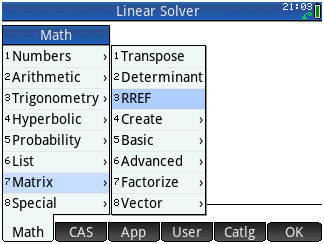
\includegraphics{Cap-ResXarxElec-Exemple-Circuit-HPP1.png}
         \item A continuació premem dos cops la combinació de tecles  
\includegraphics{HPPrime-Shift.pdf} 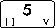
\includegraphics{HPPrime-5.pdf}; la calculadora crea una matriu buida, la qual omplirem amb la matriu $\mcmplx{Y}\ped{N}$ seguida pel vector $\mcmplx{J}\ped{N}$, creant una única matriu de quatre files i cinc columnes.

             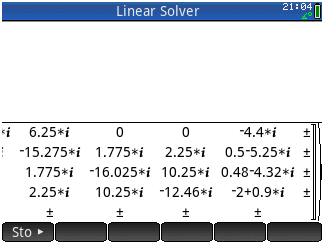
\includegraphics{Cap-ResXarxElec-Exemple-Circuit-HPP2.png}

         \item Finalment, premem la tecla 
\includegraphics{HPPrime-Enter.pdf} i la calculadora ens dona una matriu que conté la solució; les quatre primeres columnes formen una matriu identitat, i això ens indica que el sistema té solució i que és única, i la cinquena columna és la  solució buscada.

         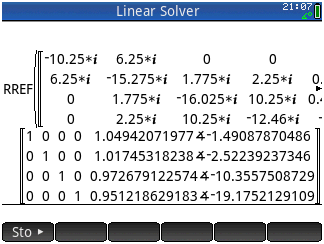
\includegraphics{Cap-ResXarxElec-Exemple-Circuit-HPP3.png}
    \end{dingautolist}

    Resoldrem ara el mateix sistema utilitzant  la funció \funsfbs{simult}; els passos a seguir són els següents:

    \begin{dingautolist}{'312}
         \item La funció \funsfbs{simult} requereix dos paràmetres, el primer és una matriu amb els coeficients del sistema, i el segon és una altra matriu amb els termes independents; d'aquesta manera, es pot resoldre alhora un mateix sistema d'equacions amb diversos conjunts de termes independents. En el nostre cas la primera matriu serà $\mcmplx{Y}\ped{N}$, i la segona, d'una columna, serà  $\mcmplx{J}\ped{N}$.

             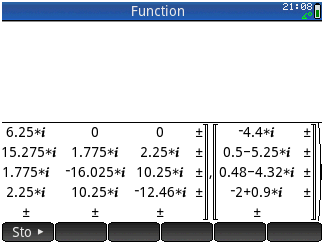
\includegraphics{Cap-ResXarxElec-Exemple-Circuit-HPP4.png}

         \item A continuació, premem la tecla 
\includegraphics{HPPrime-Enter.pdf} i la calculadora ens dona la  solució buscada.

         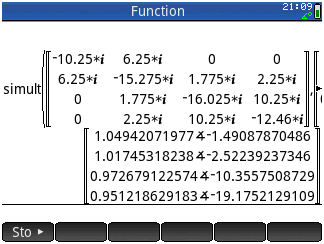
\includegraphics{Cap-ResXarxElec-Exemple-Circuit-HPP5.png}
    \end{dingautolist}
\end{exemple}


\section{Mètode particular de resolució sense acoblaments magnètics}
\index{metode@mètode dels nusos!cas particular!sense acoblaments
magnètics}

Quan no hi ha acoblaments magnètics entre branques de la xarxa, la matriu $\mcmplx{Y}\ped{N}\{n \times n\}$ i el vector $\mcmplx{J}\ped{N}\{n\}$ es poden formar de manera directa, a partir dels components de la xarxa i del seu graf orientat associat. Cal transformar també les branques d'impedància nuŀla segons la figura
\vref{pic:branca_nula}, però no és necessari fer-ho en el cas de les branques amb fonts de corrent ideals.

Per ajudar-nos en l'explicació d'aquest mètode simplificat, farem ús
del mateix exemple de la figura \vref{pic:metode_nusos}, però
suposant que no hi ha acoblament magnètic entre les branques 2 i 3
($\cmplx{X}\ped{M}=0$).

La matriu $\mcmplx{Y}\ped{N}\{n \times n\}$ i el vector $\mcmplx{J}\ped{N}\{n\}$ es formen directament tal com es descriu a continuació:

\begin{list}{}
   {\setlength{\labelwidth}{20mm} \setlength{\leftmargin}{22mm} \setlength{\labelsep}{2mm}}

   \item[$\mcmplx{Y}\ped{N}\{n \times n\}$] \index{matriu!d'admitàncies de nus $\mcmplx{Y}\ped{N}$}Matriu d'admitàncies de nus. Els elements de la diagonal estan formats per la suma de les admitàncies de les branques que incideixen en cada nus.
   Els elements de fora de la diagonal estan formats per la suma, canviada de signe, de les admitàncies de les branques que estan connectades entre cada parella de nusos.

   En el nostre exemple tenim:
   \[
      \mcmplx{Y}\ped{N} =
      \begin{pmatrix}
            \frac{1}{20} + \frac{1}{\ju 20} +  \frac{1}{10} &
            -\left[\frac{1}{20} + \frac{1}{\ju 20}\right] \\[2mm]
            -\left[\frac{1}{20} + \frac{1}{\ju 20}\right]  &
            \frac{1}{20} + \frac{1}{\ju 20} +  \frac{1}{\ju 5} + \frac{1}{10}
      \end{pmatrix}\unit{\,S} =
      \begin{pmatrix}
            \frac{3 - \ju}{20}  & \frac{-1 + \ju}{20} \\[2mm]
            \frac{-1 + \ju}{20} & \frac{3 - \ju 5}{20}
      \end{pmatrix}\unit{\,S}
   \]

   \item[$\mcmplx{J}\ped{N}\{n\}$] \index{vector!d'intensivitats de nus $\mcmplx{J}\ped{N}$}Vector
d'intensivitats de nus. Cada element d'aquest vector és format per la suma de
les intensivitats, degudes a les fonts de corrent i a les fonts de tensió, de les
branques que incideixen en cada nus; el signe de cada intensivitat és positiu si el
corrent va cap al nus, i negatiu si se n'allunya. Les fonts de tensió han de
transformar-se en fonts de corrent utilitzant l'equació \eqref{eq:Thevenin-Norton} de
la pàgina \pageref{eq:Thevenin-Norton}.

   En el nostre exemple tenim:
   \[
      \mcmplx{J}\ped{N} =
      \begin{pmatrix}
            \frac{50}{\ju 20} +  \frac{200}{10} \\[2mm]
            - \frac{50}{\ju 20} + 4
      \end{pmatrix}\unit{\,A} =
      \begin{pmatrix}
            20 - \ju \frac{5}{2} \\[2mm]
            4 + \ju \frac{5}{2}
      \end{pmatrix}\unit{\,A}
   \]

\end{list}

\index{vector!de potencials de nus $\mcmplx{V}\ped{N}$}Finalment,
calculem el vector de potencials de nus $\mcmplx{V}\ped{N}\{n\}$, tal
com  hem fet en l'apartat anterior, aplicant l'equació \eqref{eq:vn}.

En el nostre exemple tenim:
\[
   \mcmplx{V}\ped{N} = \mcmplx{Y}\ped{N}^{-1} \mcmplx{J}\ped{N} =
   \begin{pmatrix}
         \frac{3 - \ju}{20}  & \frac{-1 + \ju}{20} \\[2mm]
         \frac{-1 + \ju}{20} & \frac{3 - \ju 5}{20}
   \end{pmatrix} ^{-1}\unit{\ohm} \cdot
   \begin{pmatrix}
            20 - \ju \frac{5}{2} \\[2mm]
            4 + \ju \frac{5}{2}
   \end{pmatrix}\,\unit{A} =
   \begin{pmatrix}
         \frac{2450 + \ju 535}{17} \\[2mm]
         \frac{540  + \ju 545}{17}
   \end{pmatrix}\,\unit{V}
\]

Si volem trobar ara de forma sistemàtica totes les tensions i tots
els corrents   de les branques de la xarxa, haurem d'utilitzar
l'equació \eqref{eq:ur} de la pàgina \pageref{eq:ur} i l'equació
\eqref{eq:ir} de la pàgina \pageref{eq:ir}; això vol dir que haurem
de formar les matrius $\boldsymbol{A}$ i $\mcmplx{Y}\ped{B}$ i el
vector $\mcmplx{J}\ped{B}$. En canvi, si únicament estem
interessats en algun corrent o en alguna tensió de branca, podem
resoldre el problema aplicant les lleis de Kirchhoff a les branques
que ens interessin.

	
\begin{exemple}[\XarxaSenseAcobl{} \hyperlink{exemple:XarxaSenseAcobl}{\large\textcolor{NavyBlue}{(\faPython)}}]\label{ex:XarxaSenseAcobl}
	\addcontentsxms{\XarxaSenseAcobl}
    A partir del circuit de la figura \vref{pic:metode_nusos}, amb
    $\cmplx{X}\ped{M}=0$, es tracta de trobar els corrents que circulen
    per les branques 2 i 5.

    Partint dels potencials dels nusos 1 i 2 calculats anteriorment, i
    aplicant les lleis de Kirchhoff a les branques 2 i 5 tenim:
    \begin{align*}
       \cmplx{I}_2 &= \frac{-\cmplx{E}_2 + [\mcmplx{V}\ped{N}(1) - \mcmplx{V}\ped{N}(2)]}
                      {\cmplx{X}_2} = \frac{\qty{-50}{V} + \frac{\complexnum{2450+j535} - (\complexnum{540+
                      j545})}{17}\,\unit{V}}{\complexqty{j20}{\ohm}} = \frac{-1 - \ju 106}{34}\unit{\,A} \\[1.5ex]
       \cmplx{I}_5 &=  \frac{- \mcmplx{V}\ped{N}(2)}{R_5}  + \cmplx{J}_5 =                       \frac{\frac{\complexnum{-540-j545}}{17}\,\unit{V}}{\qty{10}{\ohm}} + \qty{4}{A} = \frac{28 - \ju 109}{34}\unit{\,A}
    \end{align*}
\end{exemple}

\section{Mètode particular de resolució amb acoblaments magnètics}
\index{metode@mètode dels nusos!cas particular!amb acoblaments
magnètics}

Quan hi ha acoblaments magnètics entre branques de la xarxa que no
tenen cap font de tensió o de corrent, també es pot aplicar el
mètode de resolució descrit en l'apartat anterior, substituint
prèviament les dues branques acoblades per un circuit equivalent
d'admitàncies, segons es veurà a continuació. 

Un cop obtingut el circuit equivalent de les dues branques acoblades
magnèticament, ja es pot formar la matriu $\mcmplx{Y}\ped{N}\{n \times n\}$ i
el vector $\mcmplx{J}\ped{N}\{n\}$, i  resoldre la xarxa tal com s'ha fet en
l'apartat anterior.

En la figura \vref{pic:equiv_acobl} es pot veure aquest circuit
equivalent.
\begin{center}
\centering
   \input{Imatges/Cap-ResXarxElec-Acoblament.pdf_tex}
   \captionof{figure}{Circuit equivalent de dues branques acoblades magnèticament} \label{pic:equiv_acobl}
\end{center}

Els valors de les admitàncies d'aquest circuit equivalent
són:\index{acoblament magnètic!circuit equivalent}

\parbox{15cm}
{ \begin{align*}
   \cmplx{Y}_{\alphaup\betaup} &= \frac{\cmplx{Z}_{\gammaup\deltaup}}{\cmplx{Z}_{\alphaup\betaup}\, \cmplx{Z}_{\gammaup\deltaup}-\cmplx{X}\ped{M}^2} &
   \cmplx{Y}_{\alphaup\gammaup} &= \cmplx{Y}_{\betaup\deltaup} = \frac{\cmplx{X}\ped{M}}{\cmplx{Z}_{\alphaup\betaup}\, \cmplx{Z}_{\gammaup\deltaup}-\cmplx{X}\ped{M}^2} \\[1.5ex]
   \cmplx{Y}_{\gammaup\deltaup} &= \frac{\cmplx{Z}_{\alphaup\betaup}}{\cmplx{Z}_{\alphaup\betaup}\, \cmplx{Z}_{\gammaup\deltaup}-\cmplx{X}\ped{M}^2} &
   \cmplx{Y}_{\alphaup\deltaup} &= \cmplx{Y}_{\gammaup\betaup} = \frac{-\cmplx{X}\ped{M}}{\cmplx{Z}_{\alphaup\betaup}\, \cmplx{Z}_{\gammaup\deltaup}-\cmplx{X}\ped{M}^2}
\end{align*} }
\hfill
\parbox{1cm}{\begin{align}\end{align}}

Un cop hem resolt la xarxa i hem trobat els potencials dels quatre
nusos $\mcmplx{V}\ped{N}(\alphaup)$, $\mcmplx{V}\ped{N}(\betaup)$,
$\mcmplx{V}\ped{N}(\gammaup)$ i $\mcmplx{V}\ped{N}(\deltaup)$, podem
trobar els dos corrents $\cmplx{I}_{\alphaup\betaup}$ i
$\cmplx{I}_{\gammaup\deltaup}$, a partir de les expressions següents:

\begin{subequations}
\begin{align}
    \cmplx{I}_{\alphaup\betaup} &=  \frac{[\mcmplx{V}\ped{N}(\alphaup) - \mcmplx{V}\ped{N}(\betaup)] \, \cmplx{Z}_{\gammaup\deltaup} - [\mcmplx{V}\ped{N}(\gammaup) - \mcmplx{V}\ped{N}(\deltaup)] \,
    \cmplx{X}\ped{M}}{\cmplx{Z}_{\alphaup\betaup}\,
    \cmplx{Z}_{\gammaup\deltaup}-\cmplx{X}\ped{M}^2} \label{eq:i_ab}
    \\[1.5ex]
    \cmplx{I}_{\gammaup\deltaup} &= \frac{[\mcmplx{V}\ped{N}(\gammaup) - \mcmplx{V}\ped{N}(\deltaup)] \, \cmplx{Z}_{\alphaup\betaup} - [\mcmplx{V}\ped{N}(\alphaup) - \mcmplx{V}\ped{N}(\betaup)] \,
    \cmplx{X}\ped{M}}{\cmplx{Z}_{\alphaup\betaup}\,
    \cmplx{Z}_{\gammaup\deltaup}-\cmplx{X}\ped{M}^2} \label{eq:i_gd}
\end{align}
\end{subequations}

El cas que hem vist  és el més general de tots els
possibles, ja que suposa que els quatre nusos $\alphaup$, $\betaup$,
$\gammaup$ i $\deltaup$ són diferents entre si. Es pot presentar el cas,
tanmateix, on dos nusos siguin en realitat el mateix, en tenir les
dues branques acoblades magnèticament, un extrem connectat al mateix
nus; en aquest cas el circuit equivalent resultant es pot derivar
del corresponent al cas general de forma senzilla.

Si suposem per exemple que les dues branques de la figura
\vref{pic:equiv_acobl} estan unides pels extrems de la dreta,
és a dir $\betaup\equiv\deltaup$, l'admitància entre
$\alphaup$ i $\gammaup$ seria $\cmplx{Y}_{\alphaup\gammaup}$, l'admitància
entre $\betaup$ i $\deltaup$ desapareixeria, l'admitància entre $\alphaup$
i $\betaup$ seria $\cmplx{Y}_{\alphaup\betaup} +
\cmplx{Y}_{\alphaup\deltaup}$, i finalment, l'admitància entre $\gammaup$
i $\betaup$ seria $\cmplx{Y}_{\gammaup\betaup} +
\cmplx{Y}_{\gammaup\deltaup}$; els corrents $\cmplx{I}_{\alphaup\betaup}$ i
$\cmplx{I}_{\gammaup\deltaup}$, es calcularien també amb les equacions
\eqref{eq:i_ab} i \eqref{eq:i_gd}, tenint en compte que
$\mcmplx{V}\ped{N}(\betaup)\equiv\mcmplx{V}\ped{N}(\deltaup)$.

\section{Circuits equivalents Thévenin i Norton} \index{teorema!de Thévenin} \index{teorema!de Norton} \index{metode@mètode dels nusos!circuits equivalents Thévenin i Norton}\label{sec:xarxes_Zth}

\index{matriu!d'impedàncies de nus $\mcmplx{Z}\ped{N}$}Per trobar el
circuit equivalent Thévenin o Norton entre dos nusos qualssevol
d'una xarxa, ens cal el vector de potencials de nus
$\mcmplx{V}\ped{N}\{n\}$, obtingut segons s'ha descrit en els
apartats anteriors, i la matriu d'impedàncies de nus
$\mcmplx{Z}\ped{N}\{n\times n\}$; aquesta matriu és definida per
la relació següent:
\begin{equation}
   \mcmplx{Z}\ped{N} = \mcmplx{Y}\ped{N}^{-1}
\end{equation}

A partir del vector $\mcmplx{V}\ped{N}$ i de la matriu
$\mcmplx{Z}\ped{N}$ podem trobar la font de tensió i la impedància
Thévenin equivalents entre dos nusos qualssevol.

La tensió Thévenin $\cmplx{E}\ped{Th}^{(\alphaup,0)}$ i la impedància
Thévenin $\cmplx{Z}\ped{Th}^{(\alphaup,0)}$, entre  un nus qualsevol
$\alphaup$ i el nus de referència 0, s'obtenen amb les equacions
següents:
\begin{align}
    \cmplx{E}\ped{Th}^{(\alphaup,0)} &= \mcmplx{V}\ped{N}(\alphaup) \\[2mm]
    \cmplx{Z}\ped{Th}^{(\alphaup,0)} &= \mcmplx{Z}\ped{N}(\alphaup,\alphaup)
\end{align}

La tensió Thévenin $\cmplx{E}\ped{Th}^{(\alphaup,\betaup)}$ i la
impedància Thévenin $\cmplx{Z}\ped{Th}^{(\alphaup,\betaup)}$, entre dos
nusos qualssevol $\alphaup$ i $\betaup$, s'obtenen amb les equacions
següents:
\begin{align}
    \cmplx{E}\ped{Th}^{(\alphaup,\betaup)} &= \mcmplx{V}\ped{N}(\alphaup) - \mcmplx{V}\ped{N}(\betaup) \\[2mm]
    \cmplx{Z}\ped{Th}^{(\alphaup,\betaup)} &= \mcmplx{Z}\ped{N}(\alphaup,\alphaup) +
    \mcmplx{Z}\ped{N}(\betaup,\betaup) - \mcmplx{Z}\ped{N}(\alphaup,\betaup) -
    \mcmplx{Z}\ped{N}(\betaup,\alphaup)
\end{align}

A partir d'aquests valors podem calcular els valors del circuit Norton equivalent, utilitzant l'equació \eqref{eq:Thevenin-Norton} de la pàgina \pageref{eq:Thevenin-Norton}.


\begin{exemple}[\XarxaThevenin{} \hyperlink{exemple:XarxaThevenin}{\large\textcolor{NavyBlue}{(\faPython)}}]\label{ex:XarxaThevenin}
	\addcontentsxms{\XarxaThevenin}
    Continuant amb el circuit de la figura \vref{pic:metode_nusos}, es
    tracta de trobar els circuits Thévenin i Norton equivalents de la
    xarxa, entre els nusos 1 i 2.

    El vector $\mcmplx{V}\ped{N}$ és el calculat a la pàgina \pageref{eq:vn_exemp}:

    \[
      \mcmplx{V}\ped{N} =
      \begin{pmatrix}
            \frac{\complexnum{15430 + j 2295}}{101} \\[2mm]
            \frac{\complexnum{3390 + j 2085}}{101}
      \end{pmatrix}\,\unit{V}
   \]

    Trobem a continuació la matriu $\mcmplx{Z}\ped{N}$, a partir de la matriu $\mcmplx{Y}\ped{N}$
    calculada a la pàgina \pageref{eq:yn}:

    \[
       \mcmplx{Z}\ped{N} =  \mcmplx{Y}\ped{N}^{-1} =
       \begin{pmatrix}
                \frac{9 - \ju 4}{60} & \frac{-3 + \ju 8}{60} \\[2mm]
                \frac{-3 + \ju 8}{60} & \frac{9 - \ju 28}{60}
          \end{pmatrix} ^{-1}\unit{\ohm} =
       \begin{pmatrix}
             \frac{1445 + \ju 310}{202} & \frac{415 + \ju 110}{202} \\[2mm]
             \frac{415 + \ju 110}{202} & \frac{245 + \ju 430}{202}
       \end{pmatrix}\,\unit{\ohm}
    \]

    Els valors del circuit Thévenin equivalent que busquem són:
    \begin{align*}
       \cmplx{E}\ped{Th}^{(1,2)} &= \frac{\complexnum{15430+j2295}}{101}\,\unit{V} - \frac{\complexnum{3390+j2085}}{101}\,\unit{V} =
       \frac{\complexnum{12040+j210}}{101}\,\unit{V} \\[2ex]
       \cmplx{Z}\ped{Th}^{(1,2)} &= \frac{\complexnum{1445+j310}}{202}\,\unit{\ohm} + \frac{\complexnum{245+j430}}{202}\,\unit{\ohm} -
       2\times\frac{\complexnum{415+j110}}{202}\,\unit{\ohm} = \frac{\complexnum{430+j260}}{101}\,\unit{\ohm}
    \end{align*}

    Els valors del circuit Norton equivalent que busquem són:
    \begin{align*}
       \cmplx{J}\ped{No}^{(1,2)} &= \frac{\cmplx{E}\ped{Th}^{(1,2)}}{\cmplx{Z}\ped{Th}^{(1,2)}} =
       \frac{\frac{\complexnum{12040+j210}}{101}\,\unit{V}}{\frac{\complexnum{430+j260}}{101}\,\unit{\ohm}} =
       \frac{\complexnum{518-j301}}{25}\,\unit{A} \\[2ex]
       \cmplx{Y}\ped{No}^{(1,2)} &= \frac{1}{\cmplx{Z}\ped{Th}^{(1,2)}} =
       \frac{1}{\frac{\complexnum{430+j260}}{101}\,\unit{\ohm}} = \frac{\complexnum{43-j26}}{250}\,\unit{S}
    \end{align*}

\end{exemple}
